\begin{block}{\textsf{Random-Neighbor} queries (\textsc{Bucketing-Generator})}
\textbf{\textsf{Random-Neighbor}}: Return a neighbor of $v$ uniformly at random.

\vspace{15pt}
\emph{\color{red}Issue:} \textsf{next-neighbor} can't jump to a random potential neighbor of $v$

\colorbox{BlueGreen}{\textbf{Bucketing}} Divide each row of the adjacency matrix into contiguous buckets

\quad$\Rightarrow$ random neighbor of $v\approx$ random neighbor in a random bucket of $v$

\vspace{15pt}

\emph{\color{red}Issue:} do \textbf{not} know $\deg(v)$; must return each neighbor with probability $1/\deg(v)$

\colorbox{BlueGreen}{\textbf{Rejection Sampling}} Return \textbf{any} neighbor with the \textbf{same} probability 

\begin{figure}[h]
    \centering
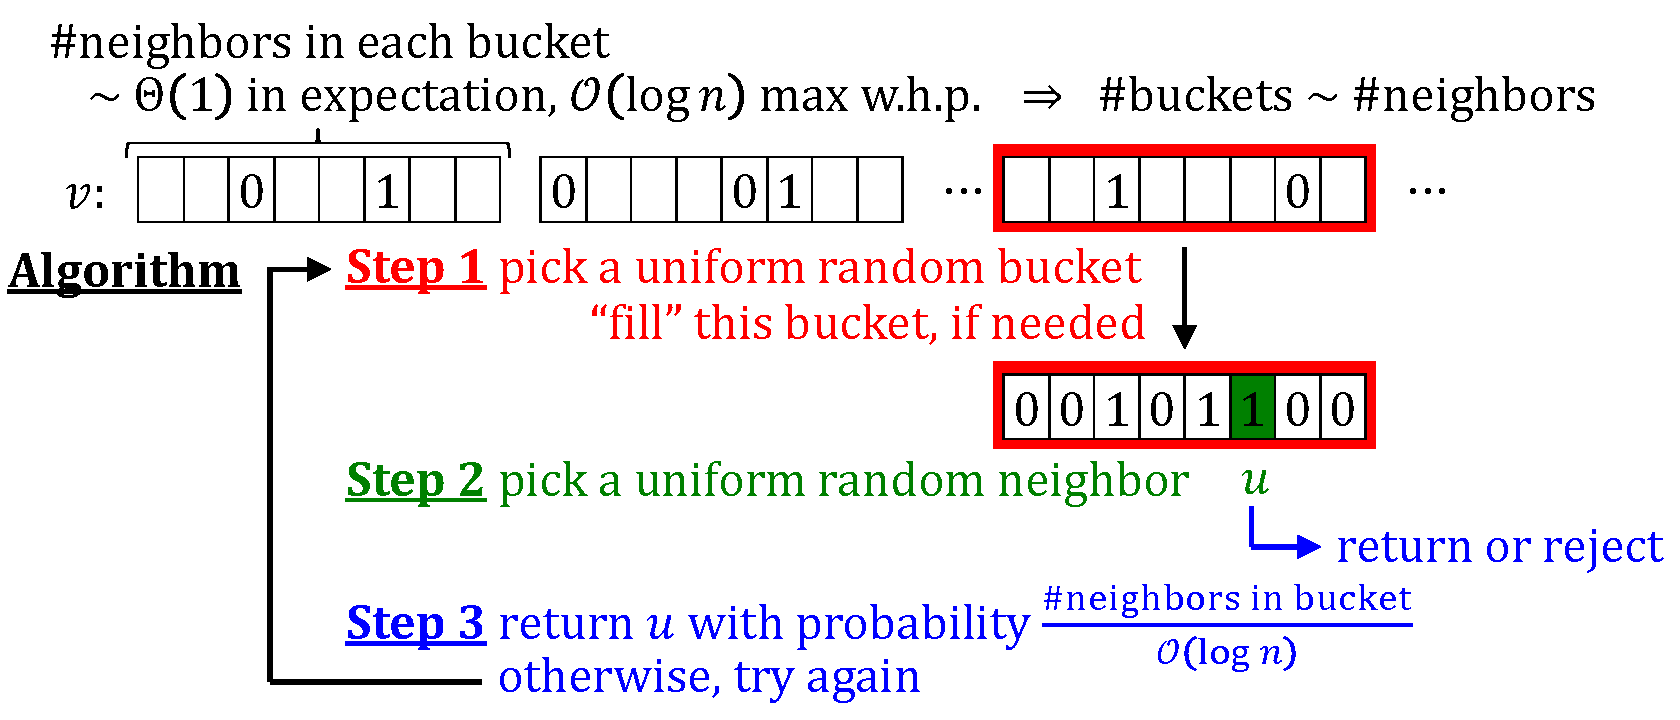
\includegraphics[clip, width=0.95\textwidth]{bckt.pdf}
\end{figure}

$\mathbb P[\textrm{return }u] = {\color{red}\frac{1}{\#\textrm{buckets}}} \times {\color{Emerald}\frac{1}{\#\textrm{neighbors in bucket}}} \times {\color{blue}\frac{\#\textrm{neighbors in bucket}}{\mathcal{O}(\log n)}}\approx\frac{\Omega(1/\log n)}{\#\textrm{neighbors of }v}$

\vspace{5pt}

$\displaystyle\mathbb P[\textrm{return any neighbor}] \approx \Omega(1/\log n) \Rightarrow$ $\mathcal{O}(\log n)$ iterations suffice

\vspace{15pt}
\colorbox{BlueGreen}{\textbf{Data Structure}} bucket maintains its known neighbors and a \textbf{filled} marker
\vspace{-8pt}
\[
  \begin{array}{l}
  \textrm{``fill'' with expected }\mathcal{O}(1)\textrm{ \textsf{Next-Neighbor} queries}\\
  \textrm{\textsf{Random-Neighbor} succeeds in }\mathcal{O}(\log n)\textrm{ tries}
  \end{array}
  \bigg\}
  \begin{array}{l}
  \mathcal{O}(\log n)\textrm{ expected time}\\
  \tilde{\mathcal{O}}(n+m)\textrm{ \emph{total} space usage}
  \end{array}
\]

%Issue: $\textsc{next-neighbor}$ can't jump to a random potential neighbor of $v$
%\begin{itemize}
    %%\item [] \textbf{Bounding the number of re-samplings:}
    %\item Divide each row of the adjacency matrix into contiguous buckets
    %\item Expected number of neighbors in a bucket is $\Theta(\log n)$
    %\item Each vertex $v$ is associated with buckets $ \langle B^v_1, B^v_2, B^v_3,\cdots\rangle$
    %\item An \textbf{unfilled} bucket may contain some indirectly exposed neighbors
    %\item A \textbf{filled} bucket will contain every possible sampled neighbor
%\end{itemize}

%%\setbeamercolor{block alerted title}{bg=Periwinkle} % Change the alert block title colors
%\begin{alertblock}{Filling the $i^{th}$ bucket $B^v_i$ of vertex $v$}
%\begin{itemize}
    %\item Use skip-sampling to produce a \textbf{potential} \emph{next-neighbor} $u$ of $v$ in $B^v_i$
    %\item Check if $(u, v)$ was set to $0$, by looking at bucket $\mathcal B$ of $u$ containing $v$
    %\item If so, re-sample. Otherwise, mark $u$ as a neighbor of $v$, and update $\mathcal B$
    %\item W.h.p, only $\mathcal O(\log^2 n)$ \textbf{potential} neighbors are generated in $B^v_i$
    %%\item With high probability, none of the buckets contain zero neighbors.
%\end{itemize}
%\end{alertblock}

\end{block}



%\vspace{-0.5in}
%%\begin{columns}[t,totalwidth=\twocolwid]

%%\begin{column}{0.49\twocolwid}

%\begin{itemize}
    %\item [] \textbf{Degree Sampling:} Sampling the degree of $v$ seems to be much harder
    %\item Sampling $deg(v)$ conditions the remaining RVs in very non-trivial ways
    %\item However, we can stil sample a random neighbor (with prob. $1/deg(v)$)
%\end{itemize}

%%\setbeamercolor{block alerted title}{bg=Periwinkle} % Change the alert block title colors
%\begin{alertblock}{$\textsc{Random-Neighbor}(v)$}
%\begin{itemize}
    %\item Choose a random bucket $\mathcal B$ of $v$. If the $\mathcal B$ is \textbf{unfilled}, fill it.
    %\item If $k$ neighbors found in $\mathcal B$, start over (reject) with probability $1-k/M$.
    %\item If accepted, return an uniformly random neighbor found in $\mathcal B$.
%\end{itemize}
%For $M = \mathcal O(\log^2 N)$, the max number of neighbors in any bucket is $<M$.
%So, the number of rejection sampling rounds is $\mathcal O(\log^2 N)$ in expectation.
%\end{alertblock}
